%\documentclass[a4paper]{article}
%\documentclass[sigconf]{acmart}
\documentclass{article}
\usepackage{nips_2018}

%\fancyhf{} % Remove fancy page headers 
%\fancyfoot[C]{\thepage}
%\setcopyright{none} % No copyright notice required for submissions
%\usepackage[small,compact]{titlesec}

\usepackage{enumitem}
%\settopmatter{printacmref=false, printccs=false, printfolios=true} % We want page numbers on submissions

%% Language and font encodings
\usepackage[english]{babel}
\usepackage[utf8x]{inputenc}
\usepackage[T1]{fontenc}

%% Sets page size and margins
%\usepackage[a4paper,top=1cm,bottom=1.5cm,left=2cm,right=2cm,marginparwidth=1.75cm]{geometry}

%% Useful packages
\usepackage{amsmath, amssymb, amsthm}
\usepackage{hyperref}
\usepackage{url}
\urlstyle{sf}
\usepackage{xcolor}
\usepackage{color}
\usepackage{balance}
% For figures
\usepackage{graphicx} % more modern
%\usepackage{epsfig} % less modern
\usepackage{subfigure} 
\usepackage{caption}
\usepackage{times}
\usepackage{natbib}
\usepackage{hyperref}
%\urlstyle{sf}
\usepackage{xcolor}
\usepackage{enumitem}
\usepackage{balance}
\usepackage{float}

\newcommand{\ak}[1]{\textcolor{blue}{\bf\small [#1 --Aleksandra]}}
\newcommand{\yd}[1]{\textcolor{violet}{\bf\small [#1 --Yatharth]}}
\newcommand{\todo}[1]{\textcolor{red}{TODO: {#1}}}
\newcommand\TODO[1]{\textcolor{red}{TODO: {#1}}}

\theoremstyle{plain}
\newtheorem{thm}{Theorem}[section]
\newtheorem{obs}{Observation}[section]
\newtheorem{lem}[thm]{Lemma}
\newtheorem{prop}[thm]{Proposition}
\newtheorem*{cor}{Corollary}
\newtheorem{defn}[thm]{Definition}

\title{The Power of The Hybrid Model for Mean Estimation}
%\author{Anonymized}

\begin{document}
\maketitle

\begin{abstract}
In this work we explore the power of the hybrid model of differential privacy (DP) proposed in~\cite{blender}, where some users desire the guarantees of the local model of DP and others are content with receiving the trusted curator model guarantees. In particular, we study the accuracy of mean estimation algorithms for arbitrary distributions in bounded support. We show that a hybrid mechanism which combines the sample mean estimates obtained from the two groups in an optimally weighted convex combination performs a constant factor better for a wide range of sample sizes than natural benchmarks. We analyze how this improvement factor is parameterized by the problem setting and how it varies with sample size. 
\end{abstract}

\section{Introduction}
Differential privacy, introduced by~\cite{dmns06}, has become the de facto standard of privacy in the computer science literature dealing with machine learning and statistical data analysis. Two traditional models of trust in the literature are: the \textit{trusted curator model (TCM)} and the \textit{local model (LM)}. In the trusted curator model, the analyst sees the true sample data and is able to calibrate the noise needed to achieve DP to the sensitivity of the query. In the local model, the analyst is only able to access samples through some locally randomizing oracle ensuring DP for each sample before it reaches the analyst. This means that each sample is received with noise calibrated to the sensitivity of the domain. It is well understood theoretically and empirically that accuracy guarantees are far better in the trusted-curator model than in the local model~\cite{kairouz2014, bassily2015local, duchi, bittau2017prochlo, fanti2016building}. Another way to phrase this is that when DP is desired in the TCM model, fewer samples are needed than in the LM. On the other hand, when it comes to deployments of DP, both companies and users find the local model of privacy better matched to their goals~\cite{wired, pew2015privacy}. This poses a challenge for companies with a smaller user bases than Apple and Google looking to deploy DP -- on the one hand, they want to guarantee local DP to their users; on the other hand, if they do, sample complexity results show they won't be able to gain much utility from the data.

Until recently in the DP community, these models were considered mutually exclusively. Recent work of~\cite{blender} observed that it may be natural and beneficial to consider a \textit{hybrid model}, in which the majority of the users desires privacy in the local model, but a small fraction of users is willing to contribute data with TCM guarantees. Indeed, it is common in industry to have a small group of ``power users" or ``early adopters" who may be willing to trust the company more than the general user~\cite{microsoft-opt-in}. % it may often be the case that some small constant fraction of the samples trust the analyst while the rest require local randomization. 
The work of~\cite{blender} demonstrates empirically that in the hybrid model one can develop algorithms that take advantage of the early adopter data in order to improve the overall accuracy of the statistics learned for the task of local search. However, their results leave open the question as to how much improvement can be gained compared with the LM, and the dependence of it on the sample size and opt-in percentage into TCM.

These are exactly the questions we aim to address in this work. In particular, we study the problem of mean estimation for arbitrary distributions in bounded support. We consider a hybrid mechanism that calculates a DP estimate of the mean of the opt-in samples (i.e., those who trust the analyst) and calculates the mean of the locally randomized samples and then outputs a convex combination of the two. We compare the performance of this hybrid mechanism with two natural benchmarks: an estimate of the mean obtained by ensuring local DP for all samples and an estimate obtained only from the opt-in samples. We characterize the outputs of these mechanisms as random variables and analyze their performance in terms of mean squared error.

We find that the hybrid mechanism outperforms the benchmarks and provide the precise characterization by how much and the dependence of the improvement on the opt-in percentage and sample size. Although the improvement factor is bounded roughly by 2, which may not seem like much, it is an encouraging finding for two reasons: first, constants matter in practical deployments of DP; and second, both the problem of mean estimation we consider and the hybrid mechanism we use are very simple. For more complex problems, where the separation in sample complexity with what's achievable in the LM and TCM is larger, and using more sophisticated hybrid mechanisms, the improvements may be significantly better. 

In Section~\ref{sec:notation} we introduce the formal notation for exploring the problem. We present analytical results describing the improvement factor and empirical results showing the performance of the hybrid mechanism against the two benchmarks in Section~\ref{sec:performance}. We conclude with a discussion of future work. Appendix~\ref{sec:preliminaries} presents the necessary mathematical background for our analysis. Appendix~\ref{sec:sample-complexity} details the technical reasons for choosing mean squared error as the accuracy metric.

%In this case, the analyst has two natural options which we will use as benchmarks against which to compare the hybrid mechanism proposed here. First, the analyst could satisfy local DP for all of the samples. Second, the analyst could use only the opt-in samples and calibrate the noise appropriately. In this work, we consider how an analyst can improve their accuracy guarantees by running a query on each population and, satisfying exactly the privacy preferences of the two populations, outputting an optimal convex combination of the two query outputs.


\section{Models and Notation}\label{sec:notation}
Each of the $n$ individuals $i \in [n]$ has data $x_i \in [0, m]$ drawn from distribution $\mathcal{D}$\footnote{We leave the question of analyzing performance when the data of opt-in and local groups comes from different distributions to future work.} with variance $\sigma^2$. The analyst only sees the original data of the $n_0 = c n$ individuals who opt-in to the trusted curator model of DP. The rest of the $n_1 = (1-c) n$ individuals prefer the local model of DP, where each individual randomizes their own data to satisfy $\epsilon$-DP and only then submits the sample to the analyst. Note that $c$ is the opt-in rate, and naturally must be bounded such that $c \in [0,1]$. Further, we expect $c$ to be small. The analyst would like to estimate the sample mean of the $n$ individuals such that each individual's trust preference is satisfied and $\epsilon$-DP is ensured. We use $\theta = \frac{1}{n}\sum_{i \in [n]}x_i$ to represent the true sample mean of all $n$ individuals. $\hat{\theta}$ will represent the analyst's $\epsilon$-DP estimate of the sample mean.

As discussed in the introduction, there are two natural benchmarks to compare with:
\begin{enumerate}
\item The fully local model in which noone opts-in to TCM, and therefore, the mechanism, which we will denote by FullLM, calculates the mean of the samples submitted to it after undergoing randomization necessary for ensuring local DP. \cite{duchi} and \cite{dky18} show that the Laplace mechanism is optimal for the problem of one-dimensional mean estimation in the local model, so wlog, we assume the samples are submitted after addition of properly calibrated Laplace noise~\cite{dmns06}. %\TODO{Do we need notation here? We don't have it, as we are careless as to whether FullLM runs on $n$ or $n_1$}
\item The model in which we ignore the data submitted in the local model, and rely only on the $n_0$ opt-in samples to calculate the DP mean, a mechanism which we will denote by OnlyTCM. We use $\theta_0 = \frac{1}{n_0}\sum_{i \in \{1, \dots, n_0\}} x_i$ to represent the true sample mean of the $n_0$ opt-in samples and $\hat{\theta}_0$ for the $\epsilon$-DP estimate of $\theta_0$ that satisfies TCM differential privacy, which we will also compute using the properly calibrated Laplace noise~\cite{dmns06}.
\end{enumerate}  

%Assuming all $n$ samples are drawn from the same distribution $\mathcal{D}$, there are two ways to perform the estimate without hybridization. FullLM preserves local $\epsilon$-DP for all $n$ samples — each individual randomizes their own data using the Laplace mechanism before submitting it to the analyst. The analyst then calculates and outputs the mean of the noisy samples. \cite{duchi} and \cite{dky18} show that the Laplace mechanism is, in fact, optimal for the problem of one-dimensional mean estimation in the local model. The second mechanism, which we call OnlyTCM, uses only the $n_0$ opt-in samples to estimate the mean of all $n$ samples and perturbs the estimate using the Laplace mechanism.

We explore how much we can improve the accuracy of our estimate by using a hybrid mechanism, which we call Hybrid. This mechanism calculates two subsample means while preserving exactly the privacy preferences of each subsample, and outputs the convex combination of the two.
%i.e., Hybrid runs OnlyTCM on the opt-in data and FullLM on the data that prefers local DP. It then outputs a convex combination of these two subsample means, giving weight $w$ to the OnlyTCM estimate and $1-w$ to the FullLM estimate. 
Specifically, let $\theta_1 = \frac{1}{n_1}\sum_{i \in \{n_0+1, \dots, n\}} x_i$ represent the true sample mean of the $n_1$ individuals who prefer LM differential privacy and $\hat{\theta}_1$ be the $\epsilon$-DP estimate of $\theta_1$ in the LM. %Note that $\hat{\theta}_1$ is obtained by running FullLM on the $n_1$ samples that prefer local randomization.
Hybrid returns an estimate $\hat{\theta} = w\hat{\theta}_0 + (1-w)\hat{\theta}_1,$ using some weight $w$, s.t., $0 < w < 1.$ We will say that the Hybrid mechanism has \textit{optimal weighing} and denote this weight by $w^*,$ if the weight minimizes the mean squared error of the estimate. We will derive $w^*$ in Lemma~\ref{lem:hybrid-error}.

%We use $\theta_0 = \frac{1}{n_0}\sum_{i \in \{1, \dots, n_0\}} x_i$ to represent the true sample mean of the $n_0$ opt-in samples and $\hat{\theta}_0$ for the $\epsilon$-DP estimate of $\theta_0$ that satisfies TCM differential privacy. Note that $\hat{\theta}_0$ is obtained by running OnlyTCM on the data. 




\section{Performance of Hybrid Mechanism}\label{sec:performance}
We now study the accuracy improvement the Hybrid mechanism provides over the benchmarks, OnlyTCM and FullLM. We study the accuracy of these mechanisms by modeling their errors as random variables and studying their expectations, in particular, their second moments about the origin. The derivations of second moments for the Laplace distribution, Normal distribution, and the Normal-Laplace distribution~\cite{Reed2006}, which are needed to compute the squared errors, can be found in Appendix~\ref{sec:preliminaries}.

\begin{lem}[Expected squared error of FullLM]
\label{MSE_FullLM}
FullLM has expected squared error
$\mathcal{E}_{\text{FullLM}} = E[(\hat{\theta} - \theta)^2] = \frac{2m^2}{n\epsilon^2}.$
\end{lem}
\begin{proof}
FullLM returns estimate $\hat{\theta} = \theta + Z/n$ where $Z$ is the sum of $n$ random variables distributed according to $Lap(m/\epsilon)$. Then clearly, $\hat{\theta} - \theta = Z/n$ and therefore, by the Central Limit Theorem (CLT), $Z \sim Nor(0, 2nm^2/\epsilon^2)$ and the lemma follows. 
\end{proof}

\begin{lem}[Expected squared error of OnlyTCM]
\label{MSE_OnlyTCM}
OnlyTCM has expected squared error
$\mathcal{E}_{\text{OnlyTCM}} = E[(\hat{\theta} - \theta)^2] = \frac{1}{cn}\left((1-c)\sigma^2 + \frac{2m^2}{cn \epsilon^2 }\right).$
\end{lem}
\begin{proof}
OnlyTCM returns the estimate $\hat{\theta} = \hat{\theta}_0$. Then we would like to study the following decomposition of the error
$\hat{\theta} - \theta = (\hat{\theta}_0 - \theta_0) + (1-c)(\theta_0 - \theta_1).$

The first term is a Laplace random variable
$\hat{\theta}_0 - \theta_0 \sim Lap\left(\frac{m}{cn\epsilon}\right).$

The second term is the difference of two sample means, so by the CLT and the difference of Normally distributed random variables
$(1-c)(\theta_0 - \theta_1) \sim Nor\left(0, \frac{(1-c)\sigma^2}{cn}\right).$

Therefore, our error follows a Normal-Laplace distribution
$\hat{\theta} - \theta \sim NL\left(0, \frac{(1-c)\sigma^2}{cn}, \frac{m}{cn\epsilon} \right).$
Thus, the conclusion follows from Lemma~\ref{nl_secmom}.
\end{proof}

\begin{lem}[Expected squared error of Hybrid]\label{lem:hybrid-error}
Hybrid has expected squared error 
$\mathcal{E}_{\text{Hybrid}} = E[(\hat{\theta} - \theta)^2] = \frac{1}{(1-c)n}\left(\frac{(w^*-c)^2\sigma^2}{c} + \frac{2(1-w^*)^2 m^2}{\epsilon^2}\right) + \frac{2m^2w^{*2}}{c^2n^2\epsilon^2},$
where
$w^* = \frac{c^2 n \left(\epsilon^2 \sigma^2+2 m^2\right)}{c \epsilon^2 n \sigma^2+2 m^2 (c (c n-1)+1)}.$
%$w^* = \frac{\frac{4 m^2}{(1-c) \epsilon^2 n}+\frac{2 \sigma^2}{(1-c) n}}{\frac{4 m^2}{c^2 \epsilon^2 n^2}+\frac{4 m^2}{(1-c) \epsilon^2 n}+\frac{2 \sigma^2}{(1-c) c n}}.$
\end{lem}

%\ak{Approximately, the optimal w is $\frac{\epsilon^2 \sigma^2+2 m^2}{\frac{\epsilon^2 \sigma^2}{c}+2 m^2}$}

\begin{proof}
We prove that $w^*$ is an optimal weighing for the convex combination of the two mean estimates, i.e., that it minimizes the mean squared error of the estimate, at the end of this proof. For now, we study the distribution of the following decomposition of the error
$\hat{\theta} - \theta = w\hat{\theta}_0 + (1-w)\hat{\theta}_1 - c\theta_0 - (1-c)\theta_1
= w\hat{\theta}_0 - c\theta_0 + (1-w)\hat{\theta}_1 - (1-c)\theta_1$
$= w(\hat{\theta}_0 - \theta_0) + (w-c)\theta_0 + (1-w)(\hat{\theta}_1 - \theta_1) + (c-w)\theta_1$
$= w(\hat{\theta}_0 - \theta_0) + (1-w)(\hat{\theta}_1 - \theta_1) + (w-c)(\theta_0 - \theta_1)$.

Each of the terms in the above equation follows a familiar distribution. In particular, the first term is simply a weight times the Laplace noise we add to the sample mean of the opt-in data. So, by Lemma \ref{wtimeslap},
$w(\hat{\theta}_0 - \theta_0) \sim Lap\left(\frac{wm}{cn\epsilon}\right).$

The second term is a weight times the sum of the Laplace noise that is added at each local randomization. Thus, by the CLT,
$(1-w)(\hat{\theta}_1 - \theta_1) \sim Nor\left(0, \frac{2(1-w)^2 m^2}{(1-c)n\epsilon^2}\right).$

The third term is the difference of two sample means, therefore, by the CLT and the difference of two Normally distributed random variables, 
$(w-c)(\theta_0 - \theta_1) \sim Nor\left(0, \frac{(w-c)^2\sigma^2}{(1-c)cn}\right).$

Putting these together, we see that our error is distributed according to the following instantiation of the Normal-Laplace distribution
$\hat{\theta} - \theta \sim NL\left(0, \frac{1}{(1-c)n}\left(\frac{(w-c)^2\sigma^2}{c} + \frac{2(1-w)^2 m^2}{\epsilon^2}\right), \frac{wm}{cn\epsilon}\right).$ The statement of the Lemma now follows from Lemma~\ref{nl_secmom}.

Now it is easy to see by taking the derivative that $w^*$ minimizes $E[(\hat{\theta} - \theta)^2].$
\end{proof}

%We can simplify the expression for $\mathcal{E}_{\text{Hybrid}}$ to $\mathcal{E}_{\text{Hybrid}} = \frac{2 c \epsilon^2 m^2 \sigma^2 (-c n+n+1)+4 m^4}{\epsilon^2 n \left(c \epsilon^2 n \sigma^2+2 m^2 (c (c n-1)+1)\right)}.$

We can now compute the improvement afforded by the Hybrid mechanism using the optimal weighting as compared to the best of the two benchmarks. %The improvement depends on several parameters because the accuracy of OnlyTCM and FullLM varies with them as per Lemmas~\ref{MSE_FullLM} and~\ref{MSE_OnlyTCM}. 

\begin{thm}[Hybrid vs. Benchmarks]\label{thm:main}
%Define $\mathcal{E}_{\text{FullLM}}$ to be $E[(\hat{\theta} - \theta)]$ where $\hat{\theta}$ is returned by FullLM and let $\mathcal{E}_{\text{OnlyTCM}}$, $\mathcal{E}_{\text{Hybrid}}$ be similarly defined.
Let $R = \frac{\min(\mathcal{E}_{\text{FullLM}}, \mathcal{E}_{\text{OnlyTCM}})}{\mathcal{E}_{\text{Hybrid}}}$.
Then, 
$$R = \gamma \cdot \frac{\epsilon^2 n \left(2 m^2 \left(c^2 n-c+1\right)+c \epsilon^2 n \sigma^2\right)}{2 c \epsilon^2 m^2 \sigma^2 (-c n+n+1)+4 m^4}, \text{where } \gamma = \min \left(\frac{2 m^2}{\epsilon^2 n},\frac{2 m^2+(1-c) c \epsilon^2 n \sigma^2}{c^2 \epsilon^2 n^2}\right).$$
\end{thm}
The proof follows from algebraic manipulation of results of Lemmas~\ref{MSE_FullLM}, \ref{MSE_OnlyTCM}, \ref{lem:hybrid-error}.

Theorem~\ref{thm:main} is difficult to interpret as it makes clear that the improvement that can be achieved by using the Hybrid approach depends on all parameters of the model: the number of samples, the opt-in rate, the distribution, the data universe, and the desired privacy parameter.

Let us first compute when $\mathcal{E}_{\text{FullLM}} \geq \mathcal{E}_{\text{OnlyTCM}}.$  Let $c_{\text{critical}} = \frac{\epsilon^2 \sigma^2}{\epsilon^2 \sigma^2+2 m^2}$ and let $n_{\text{critical}} = \frac{2 m^2}{c^2 \epsilon^2 \sigma^2+2 c^2 m^2-c \epsilon^2 \sigma^2}.$ By means of algebraic manipulation, it is easy to see that if $c>c_{\text{critical}}$ and $n \geq n_{\text{critical}}$, then $\mathcal{E}_{\text{FullLM}} \geq \mathcal{E}_{\text{OnlyTCM}}.$ %OnlyTCM has a smaller error than FullLM. 
In other words, as intuitively expected given the sample complexity results, when the opt-in rate is sufficiently large and the number of samples is sufficiently large, the DP mean estimate obtained from the opt-in samples will be more accurate than if all data was received using the LM. In this case, the improvement offered by using the Hybrid model is at most $R_{\text{max}} = \frac{2 (2-c) m^2}{(c-1) \epsilon^2 \sigma^2+2 m^2} \leq \frac{\epsilon^2\sigma^2+4m^2}{\epsilon^2\sigma^2+2m^2-1} \approx 2.$

The more interesting case, given that the motivation for the hybrid model comes from the desire to deploy DP by companies with smaller number of users, is when $n \leq n_{\text{critical}}.$ In that case, $\mathcal{E}_{\text{FullLM}} < \mathcal{E}_{\text{OnlyTCM}},$ and the factor of improvement is $R = \frac{2 m^2 \left(c^2 n-c+1\right)+c \epsilon^2 n \sigma^2 }{2 m^2 + c \epsilon^2 \sigma^2 (-c n+n+1)}.$ It is easy to check algebraically that this expression is maximized at $n = n_{\text{critical}}$ and is equal to $R_{\text{max}}.$

%$FullLM has smaller error than OnlyTCM and the factor of improvement ($R$) increases linearly with $n$. 

\begin{cor}
The maximum value of $R$ is achieved at $n_{\text{critical}}$ and is equal to $R_{\text{max}} = \frac{2 (2-c) m^2}{(c-1) \epsilon^2 \sigma^2+2 m^2}.$
\end{cor}

Figures~\ref{fig:1} and~\ref{fig:2} illustrate the relative performance of the mechanisms and the multiplicative improvement achieved by Hybrid for a particular choice of $\epsilon, m, c, \sigma^2,$ and a range of $n$.

%\TODO{The optimal weight for the convex combination depends on several parameters, such as the opt-in rate, total number of samples, the range of the support, and the privacy parameter.}

\begin{figure}[t]
%\centering
\begin{minipage}[t]{.49\textwidth}
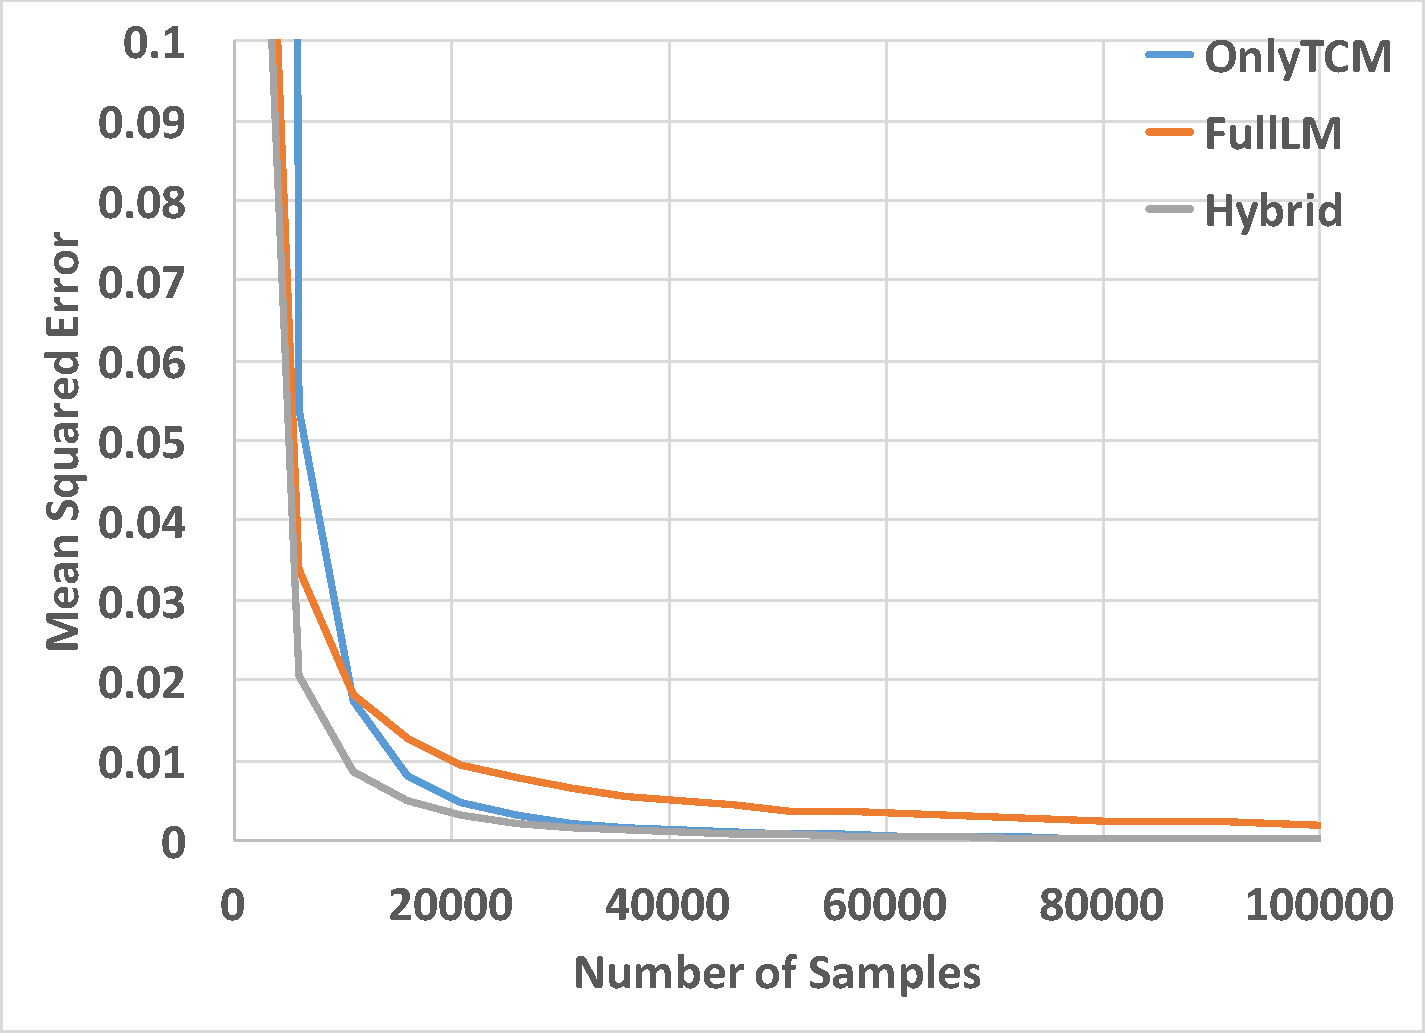
\includegraphics[width=0.99\linewidth]{eps01c01.pdf}
\caption{Relative performance of models,\\ assuming $c=0.01, \epsilon=0.1, m=1, \sigma = m/6$}
\label{fig:1}
\end{minipage}
%\end{figure}
%\begin{figure}[t]
%\centering
\begin{minipage}[t]{.49\textwidth}
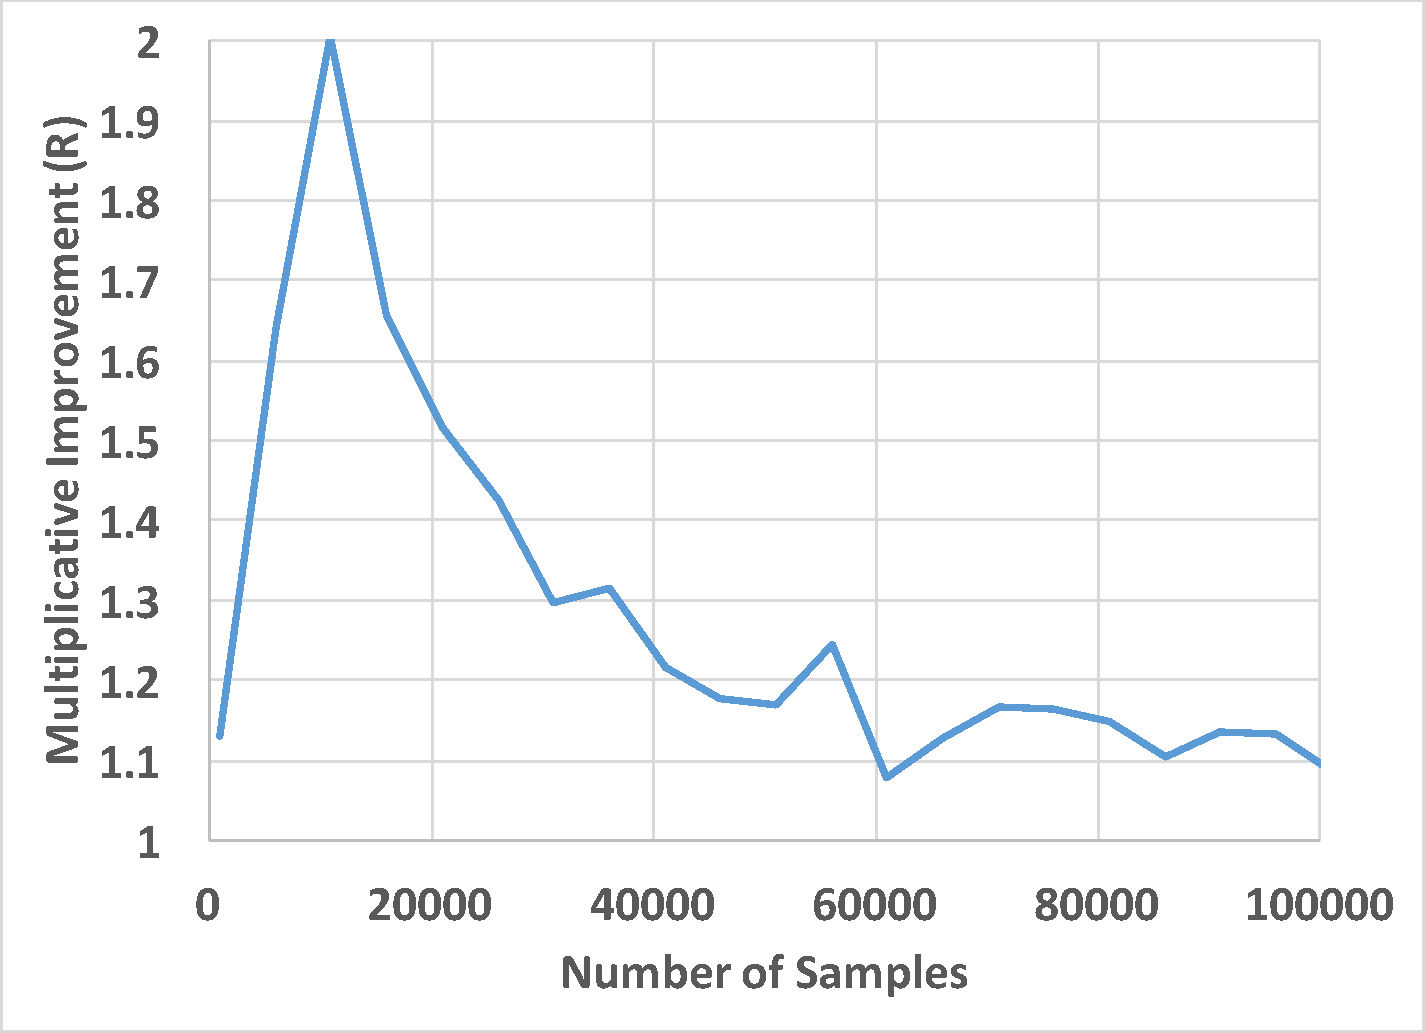
\includegraphics[width=0.99\linewidth]{imp_eps01c01.pdf}
\caption{Multiplicative improvement (R) achieved by Hybrid}
\label{fig:2}
\end{minipage}
\end{figure}

\section{Conclusions and Future Directions}
We showed that the hybrid model holds some promise for enabling wider adoption of DP by analyzing the performance of a simple hybrid mechanism for the task of mean estimation and demonstrating that in scenarios with small sample sizes it gives a lower error compared to alternatives.

%In this work, we looked at the accuracy of mean estimation algorithms in a hybrid trust environment. We propose a hybrid mechanism that calculates a DP estimate of the mean of the opt-in samples (i.e., those who trust the analyst) and calculates the mean of the locally randomized samples and then outputs a convex combination of the two. In particular, we showed that such a mechanism, where the weight of the convex combination is calculated to minimize mean squared error, can do a constant factor better for a large range of sample sizes, where the constant factor depends on several parameters.

Although for the problem of mean estimation the improvement is only a constant factor, we believe that there is additional promise in considering more sophisticated hybrid mechanisms for more complex problems. We conjecture that a hybrid mechanism that uses the opt-in samples to inform the local randomization (as done by~\cite{blender}) can significant increase utility. The conjecture stems from our analogy to the power of interactivity, where separation results between the class of problems that can be solved in the non-interactive LM and those that can be solved in the interactive LM are known~\cite{Kasiviswanathan:2011:WLP:2078965.2078976}. Thus, a natural extension to our work is to show separation for hybrid DP and local DP. % e.g., by showing that hybrid DP allows us to solve a natural variant of the masked parity problem from \cite{Kasiviswanathan:2011:WLP:2078965.2078976} that remains hard in the non-interactive local DP setting.

%Perhaps a more tractable result would be to show that hybrid mechanisms perform better than the natural benchmarks for all counting queries. \cite{Blum:2005:PPS:1065167.1065184} show that counting queries are a powerful primitive that captures a large variety of machine learning and data-mining tasks, and therefore, showing that hybrid mechanisms can improve privacy-accuracy trade-offs for this class of queries and quantifying by how much would illustrate the power and limitations that can be gained by relying on a hybrid trust model. 



%\balance
\small
\bibliography{hybrid}
\bibliographystyle{alpha}

\appendix
\section{Preliminaries}\label{sec:preliminaries}
%\section{Preliminaries}\label{sec:preliminaries}
We derive expected squared errors using the moment generating functions (mgf) of the Laplace, Gaussian, and Normal-Laplace distributions. Thus in this section, we present the relevant functions and derive the second moment about the origin for each. These expressions will then be used in calculating the expected squared errors of the mechanisms of interest in Section~\ref{sec:performance}. 

\begin{lem}[2nd moment about origin, Laplace distribution]
Let $X \sim Lap(b)$. Then, $E[X^2] = 2b^2.$
\end{lem}
\begin{proof}
The moment generating function for $X$ is $M_X(t) = \frac{1}{1 - t^2b^2}.$
Then, $M''_X(t) = -\frac{2b^2(3b^2t^2 + 1)}{(b^2t^2 - 1)^3}.$
Plugging in $t = 0$, we get 
$E[X^2] = M''_X(0) = -\frac{2b^2}{(-1)^3} = 2b^2.$
\end{proof}

The Normal random variables relevant for the work have $\mu = 0$, so we focus on the central moments of the Normal distribution.

\begin{lem}[2nd central moment about origin, Normal distribution~\cite{papoulis2002probability}]
Let $X \sim Nor(0, \sigma^2)$. Then,
$E[X^2] = \sigma^2.$
\end{lem}

We will also need to consider the error of the sum of a Laplace random variable and a Normal random variable. %Thus, characterizing the distribution of such a random variable will prove essential.
\begin{defn}[Normal-Laplace distribution~\cite{Reed2006}]
A random variable $Y \overset{d}{=} Z + W,$ where $Z \sim Nor(\mu, \sigma^2)$ and $W \sim Lap(b)$, is distributed according to the Normal-Laplace distribution, which we denote $Y \sim NL(\mu, \sigma^2, b)$.
\end{defn}

As we did with the Normal distribution above, we focus on central moments of the Normal-Laplace distribution.
\begin{lem}[2nd central moment about origin, Normal-Laplace distribution]
\label{nl_secmom}
Let $X \sim NL(0, \sigma^2, b)$. Then, 
$E[X^2] = \sigma^2 + 2b^2.$
\end{lem}
\begin{proof}
The moment generating function for $X$ is
$M_X(t) = \frac{\exp(\sigma^2t^2/2)}{1 - b^2t^2}.$
Then, as the lemma states
$E[X^2] = M''_X(0) = \sigma^2 + 2b^2.$
\end{proof}

We will also need the following property of the Laplace distribution. 
\begin{lem} \label{wtimeslap}
Let $X \sim Lap(b)$ and $Y = wX$ where $w \in [0,1]$ is a constant. Then, 
$Y \sim Lap(wb).$
\end{lem}
\begin{proof}
Let $F_X$ be the cumulative distribution function (cdf) of $X$ and $f_X$ be the probability density function (pdf) of $X$. Let $F_Y$ and $f_Y$ be the same for $Y$. Then, by definition we have 
$F_Y(y) = Pr[Y \leq y] = Pr[X \leq y/w] = F_X(y/w).$
	
Evaluating the cdf of the Laplace distribution at $y/w$, we get 
$F_X(y/w) = 
	\begin{cases} 
      \frac{1}{2}e^{\frac{y}{bw}} & y < 0 \\
      1 - \frac{1}{2}e^{-\frac{y}{bw}} & y \geq 0 
	\end{cases} .$
	
Finally, we translate the cdfs to pdfs and the lemma follows immediately, \\
$f_Y(b) = \frac{d}{dy}F_Y(y) = \frac{d}{dy}F_X(y/w) $
$= \frac{1}{2bw}
	\begin{cases} 
      e^{\frac{y}{bw}} & y < 0 \\
      e^{-\frac{y}{bw}} & y \geq 0 
	\end{cases}
     = f_X(wb).$
\end{proof}


\section{Sample Complexity Results}\label{sec:sample-complexity}
Let $\alpha$ be the accuracy parameter and $\beta$ be the confidence parameter. The following table describes the sample complexities of algorithms for mean estimation in the local model and the trusted curator model. Here the sample complexity of a mechanism is the number of samples sufficient to upper bound its absolute error by $\alpha$ with probability at least $1 - \beta$. %Note that  \cite{duchi} shows that the Laplace mechanism is optimal for one-dimensional mean estimation in both models of trust.

\begin{center}
\begin{tabular}{ |c|c|c| }
 \hline
 $\sim [0,m]$ & Sample Complexity & Optimal Algorithm~\cite{duchi} \\ [1.5ex]
 \hline
 LM & $ \frac{8}{\epsilon^2 \alpha^2} \ln\left(\frac{2}{\beta}\right)$ & Laplace \\ [1.5ex]
 \hline
 TCM & $\frac{1}{\epsilon \alpha}\ln\left(\frac{1}{\beta}\right)$ & Laplace \\ [1.5ex]
 \hline
\end{tabular}
\end{center}

The sample complexity derivation for the local model uses the concentration of the sum of i.i.d. Laplace random variables given in~\cite{chan2011private}. The sample complexity derivation for the trusted curator model comes from the accuracy statement of the Laplace mechanism in~\cite{dmns06}.

In addition to comparing the performance of hybrid mechanism with alternatives using mean squared errors, we also explored the idea of comparing them in terms of  sample complexity. This proved difficult and un-informative for several reasons. First, we found that the bound on the concentration of the sum of Laplace random variables in~\cite{chan2011private} is nice to work with analytically, but is far from tight. In addition, the inherent lack of strength of the union bound limits what we can say about errors with several terms in their algebraic expressions.

Another measure of performance we considered was absolute error. The trouble with this approach came from the difficulty in integrating one-sided probability density functions that arose from the convolution of several random variables, whether it was several Laplace random variables or a Laplace random variable and a Normal random variable. In comparison, the mean squared error was both comparatively straight-forward to calculate and gave us a precise characterization of the performance. %\TODO{Some references that in the literature absolute error and mean squared error are both used in practice?}%
\end{document}